%%%%%%%%%%%%%%%%%%%%%%%%%%%%%%%%%%%%%%%%%
% Programming/Coding Assignment
% LaTeX Template
%
% This template has been downloaded from:
% http://www.latextemplates.com
%
% Original author:
% Ted Pavlic (http://www.tedpavlic.com)
%
% Note:
% The \lipsum[#] commands throughout this template generate dummy text
% to fill the template out. These commands should all be removed when 
% writing assignment content.
%
% This template uses a Perl script as an example snippet of code, most other
% languages are also usable. Configure them in the "CODE INCLUSION 
% CONFIGURATION" section.
%
%%%%%%%%%%%%%%%%%%%%%%%%%%%%%%%%%%%%%%%%%

%----------------------------------------------------------------------------------------
%	PACKAGES AND OTHER DOCUMENT CONFIGURATIONS
%----------------------------------------------------------------------------------------

\documentclass{article}

\usepackage{fancyhdr} % Required for custom headers
\usepackage{lastpage} % Required to determine the last page for the footer
\usepackage{extramarks} % Required for headers and footers
\usepackage[usenames,dvipsnames]{color} % Required for custom colors
\usepackage{graphicx} % Required to insert images
\usepackage{listings} % Required for insertion of code
\usepackage{courier} % Required for the courier font
\usepackage{lipsum} % Used for inserting dummy 'Lorem ipsum' text into the template
\usepackage{tikz}
\usepackage{keycommand}
\usetikzlibrary{shapes}
\usepackage{amsmath}
\usepackage{mathtools}

% Margins
\topmargin=-0.45in
\evensidemargin=0in
\oddsidemargin=0in
\textwidth=6.5in
\textheight=9.0in
\headsep=0.25in

\linespread{1.1} % Line spacing

% Set up the header and footer
\pagestyle{fancy}
\lhead{\hmwkAuthorName} % Top left header
\chead{\hmwkClass : \hmwkTitle} % Top center head
\rhead{\hmwkClassInstructor} % Top right header
\lfoot{\lastxmark} % Bottom left footer
\cfoot{} % Bottom center footer
\rfoot{Page\ \thepage\ of\ \protect\pageref{LastPage}} % Bottom right footer
\renewcommand\headrulewidth{0.4pt} % Size of the header rule
\renewcommand\footrulewidth{0.4pt} % Size of the footer rule

\setlength\parindent{0pt} % Removes all indentation from paragraphs

%----------------------------------------------------------------------------------------
%	CODE INCLUSION CONFIGURATION
%----------------------------------------------------------------------------------------

\definecolor{MyDarkGreen}{rgb}{0.0,0.4,0.0} % This is the color used for comments
\lstloadlanguages{Perl} % Load Perl syntax for listings, for a list of other languages supported see: ftp://ftp.tex.ac.uk/tex-archive/macros/latex/contrib/listings/listings.pdf
\lstset{language=Perl, % Use Perl in this example
        frame=single, % Single frame around code
        basicstyle=\small\ttfamily, % Use small true type font
        keywordstyle=[1]\color{Blue}\bf, % Perl functions bold and blue
        keywordstyle=[2]\color{Purple}, % Perl function arguments purple
        keywordstyle=[3]\color{Blue}\underbar, % Custom functions underlined and blue
        identifierstyle=, % Nothing special about identifiers                                         
        commentstyle=\usefont{T1}{pcr}{m}{sl}\color{MyDarkGreen}\small, % Comments small dark green courier font
        stringstyle=\color{Purple}, % Strings are purple
        showstringspaces=false, % Don't put marks in string spaces
        tabsize=5, % 5 spaces per tab
        %
        % Put standard Perl functions not included in the default language here
        morekeywords={rand},
        %
        % Put Perl function parameters here
        morekeywords=[2]{on, off, interp},
        %
        % Put user defined functions here
        morekeywords=[3]{test},
       	%
        morecomment=[l][\color{Blue}]{...}, % Line continuation (...) like blue comment
        numbers=left, % Line numbers on left
        firstnumber=1, % Line numbers start with line 1
        numberstyle=\tiny\color{Blue}, % Line numbers are blue and small
        stepnumber=5 % Line numbers go in steps of 5
}

% Creates a new command to include a perl script, the first parameter is the filename of the script (without .pl), the second parameter is the caption
\newcommand{\perlscript}[2]{
\begin{itemize}
\item[]\lstinputlisting[caption=#2,label=#1]{#1.pl}
\end{itemize}
}

%----------------------------------------------------------------------------------------
%	DOCUMENT STRUCTURE COMMANDS
%	Skip this unless you know what you're doing
%----------------------------------------------------------------------------------------

% Header and footer for when a page split occurs within a problem environment
\newcommand{\enterProblemHeader}[1]{
\nobreak\extramarks{#1}{#1 continued on next page\ldots}\nobreak
\nobreak\extramarks{#1 (continued)}{#1 continued on next page\ldots}\nobreak
}

% Header and footer for when a page split occurs between problem environments
\newcommand{\exitProblemHeader}[1]{
\nobreak\extramarks{#1 (continued)}{#1 continued on next page\ldots}\nobreak
\nobreak\extramarks{#1}{}\nobreak
}

\setcounter{secnumdepth}{0} % Removes default section numbers
\newcounter{homeworkProblemCounter} % Creates a counter to keep track of the number of problems

\newcommand{\homeworkProblemName}{}
\newenvironment{homeworkProblem}[1][Problem \arabic{homeworkProblemCounter}]{ % Makes a new environment called homeworkProblem which takes 1 argument (custom name) but the default is "Problem #"
\stepcounter{homeworkProblemCounter} % Increase counter for number of problems
\renewcommand{\homeworkProblemName}{#1} % Assign \homeworkProblemName the name of the problem
\section{\homeworkProblemName} % Make a section in the document with the custom problem count
\enterProblemHeader{\homeworkProblemName} % Header and footer within the environment
}{
\exitProblemHeader{\homeworkProblemName} % Header and footer after the environment
}

\newcommand{\problemAnswer}[1]{ % Defines the problem answer command with the content as the only argument
\noindent\framebox[\columnwidth][c]{\begin{minipage}{0.98\columnwidth}#1\end{minipage}} % Makes the box around the problem answer and puts the content inside
}

\newcommand{\homeworkSectionName}{}
\newenvironment{homeworkSection}[1]{ % New environment for sections within homework problems, takes 1 argument - the name of the section
\renewcommand{\homeworkSectionName}{#1} % Assign \homeworkSectionName to the name of the section from the environment argument
\subsection{\homeworkSectionName} % Make a subsection with the custom name of the subsection
\enterProblemHeader{\homeworkProblemName\ [\homeworkSectionName]} % Header and footer within the environment
}{
\enterProblemHeader{\homeworkProblemName} % Header and footer after the environment
}

%----------------------------------------------------------------------------------------
%	NAME AND CLASS SECTION
%----------------------------------------------------------------------------------------

\newcommand{\hmwkTitle}{Design Document} % Assignment title
\newcommand{\hmwkDueDate}{\today} % Due date
\newcommand{\hmwkClass}{The Giving Game} % Course/class
\newcommand{\hmwkClassTime}{} % Class/lecture time
\newcommand{\hmwkClassInstructor}{University of Amsterdam} % Teacher/lecturer
\newcommand{\hmwkAuthorName}{Julian Ruger 10352783} % Your name

%----------------------------------------------------------------------------------------
%	TITLE PAGE
%----------------------------------------------------------------------------------------

\title{
\vspace{2in}
\textmd{\textbf{\hmwkClass:\ \hmwkTitle}}\\
\textmd{The Giving Game}\\
\normalsize\vspace{0.1in}\small{\hmwkDueDate}\\
\vspace{0.1in}\large{\textit{\hmwkClassInstructor\ \hmwkClassTime}}
\vspace{3in}
}

\author{\textbf{\hmwkAuthorName}}
\date{} % Insert date here if you want it to appear below your name

%----------------------------------------------------------------------------------------

\begin{document}

\maketitle

%----------------------------------------------------------------------------------------
%	TABLE OF CONTENTS
%----------------------------------------------------------------------------------------

%\setcounter{tocdepth}{1} % Uncomment this line if you don't want subsections listed in the ToC

\newpage
\tableofcontents
\newpage

%----------------------------------------------------------------------------------------
%	PROBLEM 1
%----------------------------------------------------------------------------------------

% To have just one problem per page, simply put a \clearpage after each problem

\section{1. Introduction}
I decided to create the simulator with Python(https://www.python.org/). I will be using the newest version of Python, Python 3.4, because this allows me to make use the full potential of Python.  Python is a fairly easy programming language. The syntax allows me to write the program in fewer lines of code.  With Python I do not have to specify the type of variables and the memory space is automatically allocated and deallocated. Python is also supported by alot of different packages and frameworks which can be used to write the code in even fewer lines. For example I will be using the Qt framework for the GUI. Python will save me alot of time and I only have about six or seven weeks so that is why I have chones Python. The only problem with python I might run into is the performance of the simulator. Because Python automatically allocates the memory space it might be less efficient using Python when I need to use alot of memory space. During the six/seven weeks of programming I will need to pay good attention to this problem to make sure the simulator will not get to slow at executing the tasks.

\section{2. The simulation model}
The simulator can be divided into three major parts: the algorithm implementations and the giving game itself (Back-end), the visualisation (results and graphs) and the GUI. The simulator can be seen as the following proces:

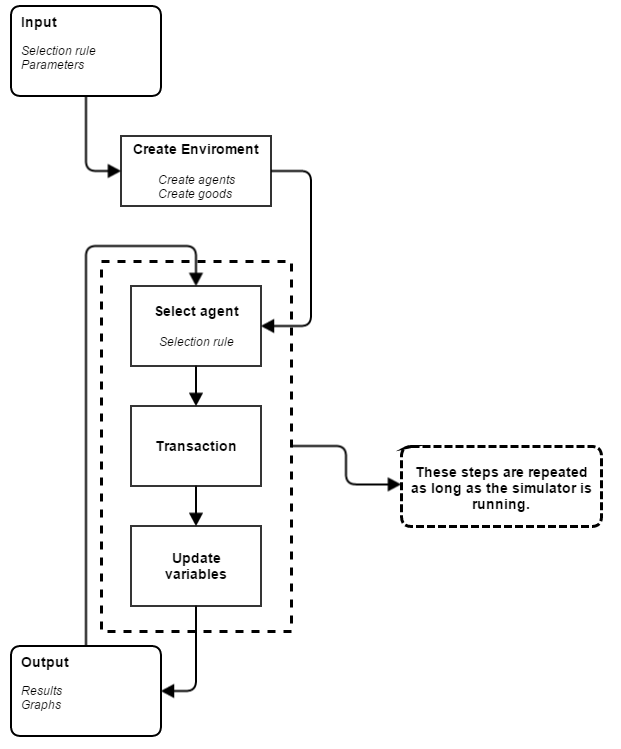
\includegraphics[scale=0.70]{Simulatorproces}


The following Input must be given to the simulator in order to get all the results (output): 
\\
\textbf{Input}

\begin{itemize}
  \item Selection rules for example the random rule, the balance rule or goodwill rule.
  \item Parameters
	\begin{itemize}
 		 \item Time, how many transactions should take place. Instead of this parameter I could also implement a start and stop button.
  		\item N number of agents
  		\item M number of goods, this parameter is not mandatory, the default number of goods will be 1.
		\item The value of the goods and if the value decreases over time.
		\item The community effect threshold with values in the range of [0, 1]. 0 meaning there is absolutely no community effect and 1 meaning that the transactions only take place in a subgroup. For example if the threshold would be 0.8 we can conclude that there is a community effect if 80/100 transactions takes place in a subgroup.
		\item The above parameter introduces another parameter. We need to determine the size of a subgroup. The size of a subgroup should be in the range of [2, x]. The value of x should be determined during the literature study.
	\end{itemize} 
\end{itemize}

\textbf{Output}

\begin{itemize}
  \item Results
	\begin{itemize}
 		 \item Community effect, depending on the given threshold can the simulator conclude if there is a community effect with a simple yes or no answer.
 		 \item The total number of transactions, balance of every agent, transactions of every agent
		 \item If a subgroup arose all the information about the agents in this subgroup should be given.
	\end{itemize} Community effect, number of transactions etc.
  \item Graphs
	\begin{itemize}
 		 \item For the community effect there should be a graph that shows the community effect over time.
 		 \item For every agant pair and good a graph should be given if the user asks for it. This might be difficult to implement, because alot of information about the agents and goods must be stored into the memory. (Yield curve)
		\item For every graph the corresponding function must be given.
	\end{itemize} 
\end{itemize}

During the development of the simulator I must take the following into account:
\begin{itemize}
  \item Multiple selection rules must already be implemented and if a new selection rule or parameter is introduced it should not be difficult to add this to the existing simulator.
 \item Every agent should keep track of all his transactions.
  \item The simulator must be able to handle a large amount of agents ranging from 1000 to a maximum of 10000 agents. 
  \item The results should be shown while the simulation is still running. If this will take too much time I could choose to only show the results if the user presses the stop/pause button.
\end{itemize}


\section{3. Back-end}
\textit{Important packages: Numpy}
\\
For every pair of agents (P, Q) we must keep track of the following things: The balance perceived by P and Q, How many times P and Q have given a good and received a good. For every single agent we must keep track of the following things: A list of all its transactions and the position of the agent (assuming an array of some sort will be used to store all the agents). For each good A and each par of agents (P, Q) we must keep track of the like factors  of each good A rangning from [-1, 0] and the value of each good A rangning from [0, $\infty$).
To accomplish the above the following design decisions have been made:
\begin{itemize}
  \item For the balance of each pair of agents (P, Q) a NxN matrix, where N is the total number of agents, will be used globally to store all the balance values of each pair.
  \item Each agent will have to store the following variables.
	\begin{itemize}
  		\item The position of the agent. For example this position is used in the NxN matrix explained above. This position will be an Integer ranging from [0, N] where N is the total number of agents.
  		\item A list of all its previous transactions. The transactions will be stored in a Python \textit{list}.
  		\item A list of the number of goods given and received for every other agent. A Numpy array will be used to store these variables. The index of the array will be the indication for each agent.
	\end{itemize}
  \item Each good will have to store the following variables.
	\begin{itemize}
  		\item The value of the good. This value is in the range of [0, $\infty$).
  		\item If the value of the good decreases over time or not. A simple True or False will be used to determine this.
	\end{itemize}
  \item For each good A a Python \textit{list} will be used globally to store each good. The size of this list will be determined by the total number of goods.
  \item For each good A and each agent P a MxN matrix, where M is the total number of goods and N the total number of agents, will be used globally to store the like factor of every good perceived by every agent.
\end{itemize}
The pseudocode below shows the decisions made above. I will use an object oriented structure to accomplish the above decisions.
\\
\textbf{Agents}
\begin{lstlisting}
from numpy import *

class Agent:
	def __init__(self, position, N):
		self.position = position
		# List of transactions, for example: [(Action, Agent, Good)] 
		# Where Action is either given or received, Agent is the agent 
		# on the other side of the transaction and Good is de good that
		# has been transfered.
		self.listoftransactions = []
		# The number of goods given and goods received for each agent
		# are stored in the variable below. For example: array([(given, received)])
		# where given is the total number of goods given to the agent 
		# with the position equal to the index and received the total number
		# of goods received from the agent.
		self.given_received = array([])
	
	def update_listoftransactions(self, new_transaction):
		self.listoftransactions.append(new_transaction)

	def give(self, receiving_agent, good):
		#The current agent gives to the receiving_agent.
		pass
	
	def receive(self, giving_agent, good):
		#The current agent receives from the giving_agent
		pass
	
	def update_given_received(self, position, previous_transaction):
		if previous_transaction == given:
			self.given_received[position][0] += previous_transaction
		elif previous_transaction == received:
			self.given_received[position][1] += previous_transaction

\end{lstlisting}
\textbf{Goods}
\begin{lstlisting}
class Goods():
	def __init__(self, value, decreasing)
		self.value = value # The value of the good
		self.decreasing = decrasing # Either True or False

	def decrease(self, decreasing_factor):
		self.value = self.value * decreasing_factor
\end{lstlisting}
\clearpage
\textbf{Creating the Giving Game enviroment}
\begin{lstlisting}
import Agents
import Goods
# A different file should contain all the functions for the selectio rules.
# Each selection rule will have one function, this function is called before
# every transaction.
import Selectionrules

def create_agents(N):
	# Create N agents by calling the __init__() from the Agents Class
	pass

def create_goods(M):
	# Create M product by calling the __init_() from the Goods Class
	pass

def transaction(P, Q):
	# Start a transaction between P and Q by calling give() and receive() 
	# from the Agents Class 
	# P give to Q
	P.give(Q)
	# Q reveives from P
	Q.receive(P)

def update_balancematrix(balancematrix):
	# Update the balance matrix after every transaction
	pass

def select_agent(selectionrule):
	# Call the right seletion rule to select the agent
	pass

def main():
	create_agents(N)
	create_goods(M)
	# Start the game 
	P = current_agent #Choose a random agent
	While(Start):
		Q = select_agent(selectionrule)
		transaction(P, Q, good)
		P = Q

if __name__ == '__main__':
    main()


\end{lstlisting}

\section{4. Visualisation}
\textit{Important packages: Numpy, matplotlib, PyChart}
\\
With Either \textit{matplotlib} or \textit{PyChart} I can plot graphs. I will start with \textit{matplotlib}, because this package is better documented and can be used together with the Qt framework which I will be using for the GUI. Together with \textit{Numpy} I will be able to do all the necessary calculations and produce together with the Qt framework well formatted results.
\section{5. GUI}
\textit{Important packages: VisPy}
\textit{Important framwork: Qt}
For the GUI I will be using the Qt framework. 
\\
The GUI for the input of a few parameters will look something like this:

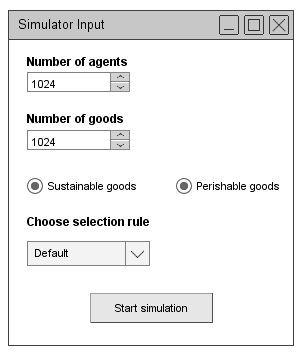
\includegraphics[scale=0.70]{Inputexample}

The results will look something like this:

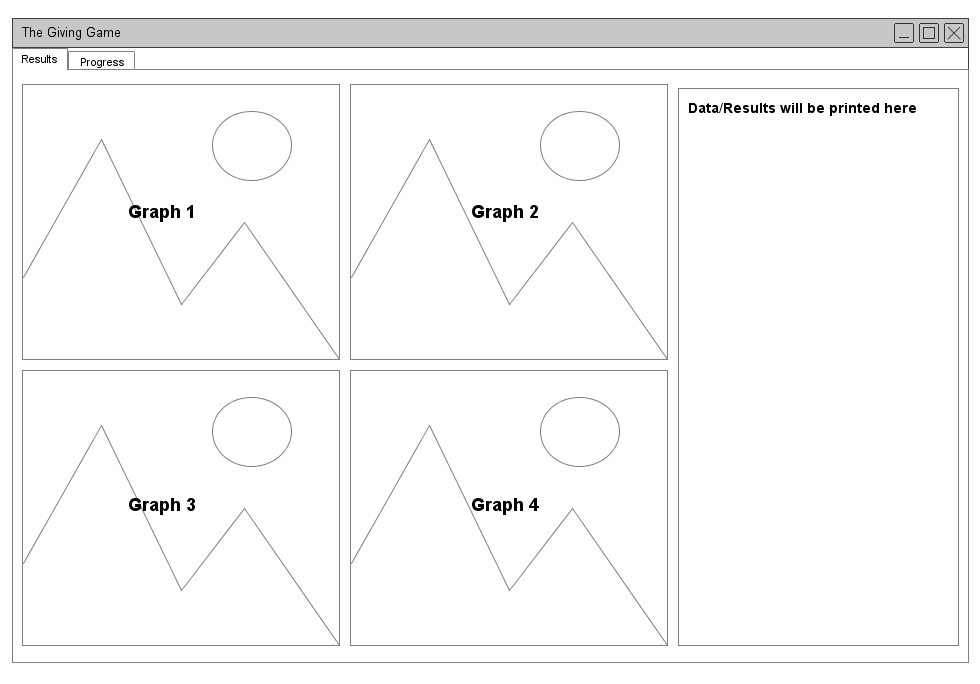
\includegraphics[scale=0.70]{Resultsexample}

The second tab will be used to show the following:

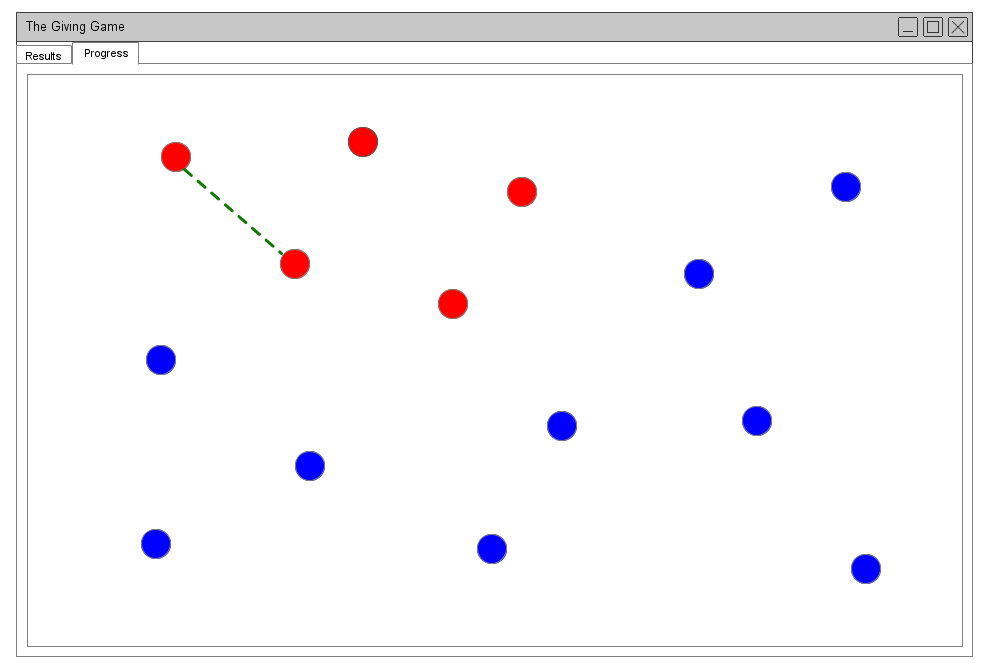
\includegraphics[scale=0.70]{Progressexample}

Here the user can see the progress of the giving game. The green dotted line shows a transaction. The color shows the subgroups. For example red could mean that the transactions take most of the time place in this subgroup and blue would mean the opposite. This visualisation of the progress will be implemented last. For this part of the visualisation I will be needing \textit{OpenGL}. To accomplish this I will be making use of the package \textit{VisPy}.

\section{6. Possible additions}
\begin{itemize}
  \item I could add a variable for the most traded goods and base the results more on the goods to see how different kind of goods affect the results. 
\end{itemize}

\section{7. Changes and Updates}
\textbf{Goods}
\begin{itemize}
  \item The perish factor is now called the perish period because it is a natural number in the interval [0, $\infty$ ). These values are more logical if we think of time
  \item The production time is now called the production delay. This delay is a natural number in the interval [0,  $\infty$). The production delay starts when the good has perished.
\end{itemize}





%----------------------------------------------------------------------------------------

\end{document}